% Pacchetti richiesti nel preambolo del main.tex per la corretta compilazione di questo capitolo:
% \usepackage{tikz}
% \usetikzlibrary{shapes.geometric, positioning, arrows.meta, calc, decorations.pathreplacing}

\chapter{Gestione delle Transazioni nelle Basi di Dati Distribuite}

\section{Architetture e Tipologie di Transazioni Distribuite}

Il mondo reale dei sistemi informativi complessi richiede di trascendere l'isolamento del singolo calcolatore. L'architettura evolve verso il concetto di \textbf{Base di dati distribuita}.
In un tale paradigma, il patrimonio dei "dati e il controllo sono distribuiti su server (nodi) diversi, coordinati fra loro". L'insieme omogeneo forma un dominio logico (indicato con $D$) entro il quale le operazioni della transazione $T$ in ingresso "sono per quanto possibile delegate ai vari nodi" per favorire il parallelismo e la vicinanza geografica o logica al dato.

\vspace{1em}
\begin{center}
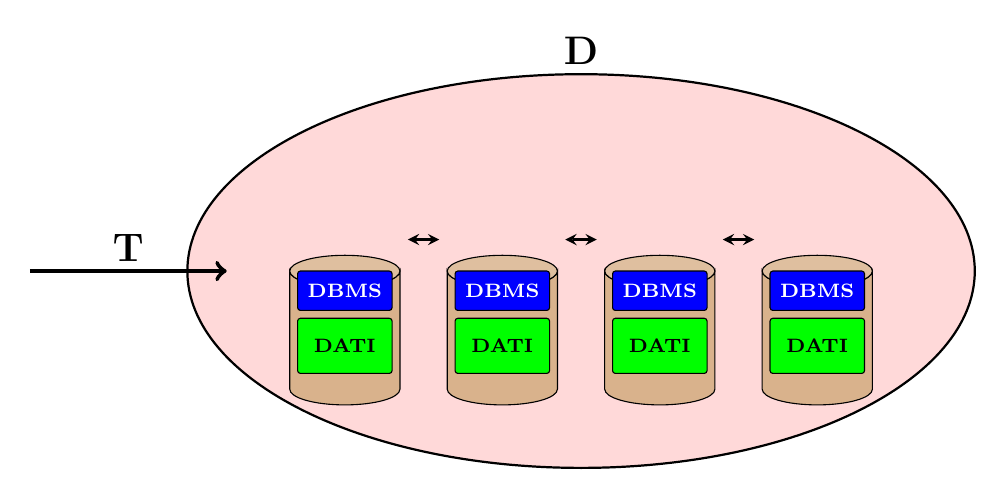
\begin{tikzpicture}
% Contorno del dominio D
\draw[thick, fill=red!15] (4,0) ellipse (5cm and 2.5cm);
\node at (4,2.8) {\Large \textbf{D}};

% Nodi
\foreach \x/\name in {1/A, 3/B, 5/C, 7/D} {
    \begin{scope}[shift={(\x,-0.5)}]
        % Cilindro di base (colore marrone chiaro)
        \draw[fill=brown!60] (-0.7,-1) -- (-0.7,0.5) arc (180:360:0.7cm and 0.2cm) -- (0.7,-1) arc (360:180:0.7cm and 0.2cm);
        \draw[fill=brown!50] (0,0.5) ellipse (0.7cm and 0.2cm);

        % Blocco DBMS
        \draw[fill=blue, rounded corners=1pt] (-0.6,0) rectangle (0.6,0.5);
        \node[text=white, font=\scriptsize] at (0,0.25) {\textbf{DBMS}};

        % Blocco DATI
        \draw[fill=green, rounded corners=1pt] (-0.6,-0.1) rectangle (0.6,-0.8);
        \node[text=black, font=\scriptsize] at (0,-0.45) {\textbf{DATI}};
    \end{scope}
}

% Frecce di coordinamento tra i nodi
\draw[stealth-stealth, thick] (1.8, 0.4) -- (2.2, 0.4);
\draw[stealth-stealth, thick] (3.8, 0.4) -- (4.2, 0.4);
\draw[stealth-stealth, thick] (5.8, 0.4) -- (6.2, 0.4);

% Freccia di ingresso T
\draw[->, ultra thick] (-3, 0) -- (-0.5, 0);
\node at (-1.75, 0.3) {\Large \textbf{T}};

\end{tikzpicture}
\end{center}
\vspace{1em}

Le strategie per l'implementazione pratica di queste "Architetture per basi di dati distribuite" si basano su due tecniche cardinali (spesso sovrapposte):
\begin{itemize}
    \item \textbf{Partizionamento (sharding)}: Consiste nella "suddivisione dei dati fra vari nodi". Una gigantesca tabella, ad esempio, viene segmentata orizzontalmente in \textit{chunk} o porzioni assegnate a macchine indipendenti per bilanciare il carico I/O.
    \item \textbf{Replicazione}: Consiste nel mantenere gli "stessi dati su più nodi" per ridondanza, fault-tolerance o per avvicinare i record in lettura agli utenti dislocati nel globo.
\end{itemize}

A livello applicativo, i linguaggi come SQL si adattano alla topologia di rete gestendo due ordini di interazioni:
\begin{enumerate}
    \item \textbf{Transazione Remota}: Avviene quando un client esegue un programma che necessita di "Interagire con una base di dati nel contesto di un'altra". In SQL (standard Oracle/dblink), la sintassi esplicita la deviazione verso un nodo esterno tramite l'operatore \texttt{@}. Esempio:
\begin{verbatim}
UPDATE scott.dept@sales.us.americas.acme_auto.com
SET loc = 'NEW YORK' WHERE deptno = 10;
\end{verbatim}
    \item \textbf{Transazione Distribuita su più basi di dati (o su base frammentata)}: Avviene quando l'applicativo mira a "Interagire con più basi di dati contemporaneamente" o frammentate all'interno di una singola unità logica di lavoro ("La distribuzione è spesso trasparente per l'utilizzatore"). In questo caso la transazione spara direttive a tabelle diverse gestite da motori paralleli, per poi imporre una chiusura globale:
\begin{verbatim}
UPDATE scott.dept SET loc = 'NEW YORK' WHERE deptno = 10;
UPDATE scott.emp SET deptno = 11 WHERE deptno = 10;
COMMIT;
\end{verbatim}
\end{enumerate}

\section{Tecnologia, Consistenza e Durabilità nei Sistemi Distribuiti}

Focalizzandosi prettamente sui "contesti con il solo sharding" puro (l'analisi della replicazione introduce logiche differenti), l'architettura a rete dimostra un'intrinseca modularità: "la distribuzione non influenza consistenza e durabilità".
Questo postulato si declina per i singoli gestori atomici:
\begin{itemize}
    \item \textbf{Consistenza Locale}: "La consistenza non dipende dalla distribuzione: i vincoli di integrità sono locali". Poiché "la tecnologia DBMS attuale non gestisce vincoli distribuiti" incrociati o foreign key tra server fisici disgiunti, il gestore di integrità di ogni nodo si limita a vigilare asetticamente sulla conformità del proprio frammento locale di dati.
    \item \textbf{Durabilità Locale}: Analogamente, "La durabilità non dipende dalla distribuzione: ogni sistema garantisce la durabilità locale utilizzando meccanismi di recupero locali". Ciascun DBMS partecipante scrive diligentemente il proprio "log", stacca il proprio "checkpoint" e crea il proprio "dump" su dischi fisici locali.
\end{itemize}

Ciò che risulta drammaticamente ed esclusivamente impattato (e che rappresenta l'"Aspetto rilevante") dalla natura distribuita è la triade composta da:
\begin{enumerate}
    \item **Concorrenza** (e isolamento relazionale).
    \item **Affidabilità** (esclusivamente intesa come tutela dell'atomicità "tutto o niente" a livello macroscopico).
    \item **Ottimizzazione delle interrogazioni** (efficienza del piano di esecuzione di rete).
\end{enumerate}

\section{Controllo di Concorrenza su Nodi Plurimi}

Nel contesto distribuito, l'isolamento diviene un'astrazione fragile.
"In teoria: La serializzabilità locale non è sufficiente per la serializzabilità globale".

Si esamini il seguente "Esempio, due transazioni $t_1$ e $t_2$ su due nodi A e B":
$$t_1: r_{1A}(x) \ w_{1A}(x) \ r_{1B}(y) \ w_{1B}(y)$$
$$t_2: r_{2B}(y) \ w_{2B}(y) \ r_{2A}(x) \ w_{2A}(x)$$
Se i due nodi fossero svincolati l'uno dall'altro, ciascuno schedulerebbe autonomamente i propri task. Potrebbero emergere i seguenti schedule fisici "Sui nodi":
$$\text{Nodo A}: r_{1A}(x) \ w_{1A}(x) \ r_{2A}(x) \ w_{2A}(x)$$
$$\text{Nodo B}: r_{2B}(y) \ w_{2B}(y) \ r_{1B}(y) \ w_{1B}(y)$$
Analizzandoli separatamente, il nodo A garantisce l'isolamento locale serializzando $t_1$ prima di $t_2$ (Conflict-equivalente a $t_1 \to t_2$). Il nodo B agisce altrettanto lecitamente sul suo frammento $y$, ma serializza $t_2$ prima di $t_1$ (Conflict-equivalente a $t_2 \to t_1$). Sebbene i due DB siano singolarmente perfetti e privi di lock falliti, il collante logico intersistemico è spezzato: l'ordine dei conflitti R-W si è capovolto. Il sistema non possiede serializzabilità globale, esponendo la business logic ad anomalie gravissime.

"Però", nella prassi architetturale, il disastro si sventa facilmente.
Il rispetto del protocollo S2PL (Strict Two-Phase Locking) salva il paradigma: "se i lock in scrittura sono mantenuti fino al commit, che è globale (cioè coinvolge tutti i nodi) la serializzabilità è garantita dall'ordinamento dei commit e dalle letture delle versioni appropriate". Inibendo il rilascio di un lucchetto su A finché B non ha pattuito la chiusura collettiva, lo scheduler forza in stallo (o a risoluzione topologica corretta) ogni tentativo di inversione cronologica asincrona.

\section{Guasti Sistemici e l'Atomicità Globale}

Il problema monumentale della base di dati distribuita emerge durante il \texttt{commit}. Per tutelare l'atomicità ("tutto o niente") della transazione globale, un fallimento in un singolo frammento allocato a Tokyo deve potersi riversare, annullando retroattivamente e inesorabilmente i calcoli di successo già elaborati nel frammento allocato a Roma.

A peggiorare le probabilità di successo intervengono i "Guasti nei sistemi distribuiti":
\begin{itemize}
    \item \textbf{Guasti sui singoli nodi (locali)}: Equiparabili al "caso centralizzato" (crash di sistema locale, blackout).
    \item \textbf{Perdite di messaggi}: L'instabilità del cavo di rete corrompe i pacchetti TCP/IP. Le perdite "lasciano i protocolli in stato di incertezza". Per prassi, "I messaggi sono seguiti da conferme (ack)". Purtroppo, nell'alveo dell'affidabilità "Si possono perdere gli uni come gli altri" generando loop di retrying o false deduzioni di down.
    \item \textbf{Partizionamento della rete}: Uno switch principale cade e la rete si spacca in due emisferi ciechi tra di loro, pur mantenendo i nodi interni vivi e vitali.
\end{itemize}

Per governare questo caos comunicativo si elegge un paradigma rigido ad "Una decisione (commit o abort) per tutti i partecipanti ad una transazione".

Questa concertazione è "Simile ad un contratto" notarile civile:
"Due o più parti si impegnano e una terza parte (il mediatore o il notaio) ratifica" la validità formale dell'atto.
Gli attori sul palcoscenico informatico assumono nomenclature speculari:
\begin{itemize}
    \item \textbf{I partecipanti}: Nodi foglia che detengono la frazione dei dati. Assumono il ruolo di \textit{resource manager} (RM).
    \item \textbf{Il coordinatore}: Il nodo centrale (spesso eletto tra uno stesso dei partecipanti, non necessariamente un server a parte) che orchestra i turni. Assume il ruolo di \textit{transaction manager} (TM).
\end{itemize}

\section{Il Protocollo di Commit a Due Fasi (2PC)}

Il meccanismo sincronico universale atto a preservare l'atomicità diffusa è il \textbf{Protocollo di commit a due fasi}. Esso ricalca la cerimonia nuziale: prima si interpellano le parti individualmente, si acquisisce l'eventuale assenso vincolante e, solo a seguito dell'unanimità, si proclama l'atto pubblico o l'annullamento.

Esistono "Due fasi, preparazione e conferma, separate da una decisione" irrevocabile e centrale.
\begin{itemize}
    \item \textbf{Fase di preparazione}: Il TM interroga la platea lanciando il quesito "siete disponibili al commit?".
    \item \textbf{Momento di decisione}: "se tutti d'accordo 'ok' altrimenti 'lasciamo perdere'".
    \item \textbf{Fase di conferma}: Consta della "comunicazione a tutti, con conferma di ricezione" dell'esito, per forzare l'allineamento dei dischi.
\end{itemize}
Questo balletto diplomatico si regge integralmente "con scambio (rapido) di messaggi fra coordinatore e partecipanti con scritture nei log e con conferme (ack)" ad ogni singolo step per garantirsi la persistenza logica a fronte dei guasti di rete.

\subsection{Dizionari di Log: TM vs RM}
Il rigore protocollare si evince dai vocaboli esatti che i manager incedono e marchiano in memoria stabile.

\textbf{Record nel log del coordinatore (TM)}:
\begin{itemize}
    \item \texttt{prepare}: Marcatore primordiale. "Contiene l'identificatore della transazione e dei partecipanti". Costituisce il promemoria fisico, "serve a ricordare di avere chiesto disponibilità".
    \item \texttt{global commit} o \texttt{global abort}: Rappresentano l'istante cogente della "decisione".
    \item \texttt{complete}: Atto di chiusura che segna la "conclusione del protocollo" e permette di scartare i file in ram.
\end{itemize}

\textbf{Record nei log dei partecipanti (RM)}:
Oltre alle tracce abituali "come già visto per la gestione tradizionale: begin, insert, delete, e update oltre a commit e abort", viene forgiato un record rivoluzionario:
\begin{itemize}
    \item \texttt{ready}: È la cambiale e la "conferma di avere dato disponibilità (irrevocabile) a partecipare al commit; contiene riferimenti alla transazione e al coordinatore". Questo record viene scritto dal frammento \textit{solamente} "dopo avere verificato che, dal punto di vista del partecipante, la transazione può andare in commit (ha le risorse, soddisfa i vincoli,...)".
    L'atto di firma per l'RM è un suicidio tattico temporaneo: "dopo aver scritto ready il partecipante perde la propria autonomia decisionale sulla transazione". A prescindere da blackout futuri, per lui quel pacchetto di record è congelato in pendenza perpetua.
\end{itemize}

\subsection{Evoluzione Completa delle Due Fasi}

\textbf{Prima Fase del Protocollo (Preparazione):}
\begin{enumerate}
    \item "Il coordinatore scrive \texttt{prepare} (indicando transazione e partecipanti) nel log e poi invia un messaggio di \texttt{prepare} ai partecipanti. Fissa un timeout per le risposte". (Sveglia 1).
    \item "Ogni singolo partecipante che riceve il messaggio di \texttt{prepare}" valuta la sua coscienza logica.
    \item "se è in grado di partecipare al commit, scrive nel proprio log un record di \texttt{ready} e poi trasmette al coordinatore un messaggio di \texttt{ready} per comunicare la propria disponibilità".
    \item "altrimenti, può inviare un mesaggio di \texttt{not-ready} (oppure niente)", rifugiandosi nel silenzio.
    \item "Il coordinatore riceve risposte fino al timeout".
    \item "se ha ricevuto \textit{tutte} le risposte e sono \textit{tutte positive} scrive un record \texttt{global commit} nel proprio log". L'atomicità in positivo è sancita.
    \item "altrimenti (almeno una risposta mancante o negativa) scrive un record di \texttt{global abort}". La catena si frantuma per salvaguardare l'insieme.
\end{enumerate}

\textbf{Seconda Fase del Protocollo (Conferma e Propagazione):}
\begin{enumerate}
    \item "Il coordinatore trasmette la decisione (globale) ai partecipanti che hanno risposto \texttt{ready} e a quelli la cui risposta non è arrivata, fissando un nuovo time-out". (Sveglia 2).
    \item "Ogni partecipante che riceve il messaggio, scrive la decisione (record di \texttt{commit} o \texttt{abort}) nel proprio log, invia un ack al coordinatore e implementa la decisione con le opportune scritture" (rilasciando lucchetti 2PL ecc.).
    \item "Il coordinatore riceve i messaggi di ack dai partecipanti".
    \item "se allo scadere del time-out ne manca qualcuno (fra coloro che avevano risposto \texttt{ready} o non avevano risposto), invia loro di nuovo la decisione". (Insiste fino alla sfinimento).
    \item "quando tutti hanno risposto scrive un record di \texttt{complete} nel log". Protocollo estinto.
\end{enumerate}

\section{Stati Anomali: La Finestra di Incertezza e il Recovery Distribuito}

Il nervo scoperto ed il punto debole intrinseco del 2PC risede nello stato liminale del RM.
"Un partecipante in uno stato di \texttt{ready}" ha letteralmente e volontariamente "perso la propria autonomia". Esso "attende la decisione del coordinatore" centrale.
Tuttavia, "se ha acquisito lock (e questo accade quasi sempre) le risorse relative sono bloccate" a tempo indeterminato e "è lasciato in uno stato incerto in caso di fallimento del coordinatore".

Questo lasso di tempo psicologico e formale si definisce **Finestra di incertezza**. Corrisponde a "l'intervallo tra la scrittura del \texttt{ready} e la ricezione della decisione". Durante questi secondi (o ore, in caso di crash prolungato del nodo leader), "il partecipante resta in attesa della decisione e non può fare niente". Non può dedurre un abort arbitrario (potrebbe innescare un'anomalia globale se il leader aveva già ratificato il global commit su altri nodi), né tantomeno forzare il salvataggio. Resta congelato.

\subsection{Recupero Post-Crash (Recovery del TM e dell'RM)}
I "Guasti (Crash, perdite di messaggi di notifica o di ack, partizionamenti)" vengono sterilizzati ed incapsulati col dogma pessimista: "sono gestiti tutti nello stesso modo: se non si riceve conferma si considera fallita la fase".
Conseguenze immediate per l'orchestratore TM: "se è la prima, (di solito) si abortisce; se è la seconda, si ripete la seconda fase". ("Nota bene: la decisione è presa fra la prima e la seconda fase, quindi la seconda fase non può modificarla", è solo uno sforzo di propagazione e notifica).

Al risveglio dopo un blackout severo o un boot a freddo, i motori eseguono lo scanning dei propri archivi fisici stabili:

**Recovery (ripristino) di un partecipante (RM):**
L'agente isolato sonda "Per ogni transazione" pendente.
\begin{itemize}
    \item "se l'ultimo record nel log relativo ad essa è un \texttt{commit}, le sue azioni debbono essere confermate (redo)". La catena locale è conclusa.
    \item "se l'ultimo record è un'azione o un \texttt{abort}, allora la transazione deve abortire, con undo delle sue azioni". Significa che il partecipante è "caduto" prima ancora di spedire la dichiarazione di ready. Essendo mancata la sua risposta al giro primario, il TM avrà dedotto l'aborto per l'intero grappolo. Procedere all'undo locale è perfettamente coerente col diktat globale.
    \item "se l'ultimo record è un \texttt{ready}, il partecipante non ha informazioni sull'esito della transazione e ha bisogno di notizie dal coordinatore". Il partecipante si trova bloccato nella maledetta finestra. Non vi è algoritmo locale salvifico: "può aspettare o chiederle". Interrogherà il master al suo risveglio.
\end{itemize}

**Recovery (ripristino) del coordinatore (TM):**
Rialzatosi dalle proprie ceneri, il leader valuta la sua coda "Per ogni transazione" in base all'ultimo fiato vitale apposto nel log.
\begin{itemize}
    \item "se l'ultimo record è \texttt{complete}, non è necessario fare niente (la decisione è stata presa e tutti sono stati informati e hanno recepito l'informazione)". Pratica evasa.
    \item "se l'ultimo record è una decisione (\texttt{global commit/abort}), allora la decisione è stata presa e non può essere cambiata, ma non è sicuro che tutti siano informati e allora va ripetuta la seconda fase". Il TM spara massivamente nel brodo primordiale i solleciti fino a esaurire tutti gli ack dei dispersi.
    \item "se l'ultimo record è \texttt{prepare}, ci possono essere partecipanti in attesa della decisione" sparsi nell'etere. Ma non essendo approdato al global commit prima della morte, "la soluzione più semplice è global abort" (cancellare tutto l'albero d'impegno), o in alternativa (se si presume che i dati siano vivi), "è possibile ripetere la prima fase" rilanciando le interrogazioni.
\end{itemize}
